\chapter{Background}
\newacronym{SQL}{$SQL$}{Structured Query Language}
\glsadd{SQL}
\newacronym{UART}{$UART$}{Universal Asynchronous Receiver-Transmitter}
\glsadd{UART}
\newacronym{URL}{$URL$}{Uniform Resource Locator}
\newacronym{GPIO}{$GPIO$}{General Purpose Input Output}
\glsadd{GPIO}
\newacronym{I2C}{$I2C$}{Inter-Integrated Circuit}
\glsadd{I2C}
\newacronym{SPI}{$SPI$}{Serial Peripheral Interface}
\glsadd{SPI}
\newacronym{DOM}{$DOM$}{Document Object Model}
\glsadd{DOM}
 
 
The monitoring system is split into three different parts which includes the web application, Raspberry Pi and the cloud(Azure). These are also split into their respective parts with the web application containing the web server(node) and the website(React), the Cloud; AzureSQL server and AzureSQL database, the Raspberry Pi; flask server, the fingerprint and the \gls{RFID}. These terms are used in the Designs and Implementation section of this Literature.
 
\section{Web Application}
A website is often confused with a web page, a web application or a web server. According to MozillaWebDoc, A website is a collection of web pages which are grouped together in various ways. A web server is a computer that hosts websites and their supporting files, which are available on that computer. A web application is a software that can be accessed using a web browser.\cite{Whatisth32:online} It is designed for authorised users to interact with a particular resource or service. Authentication is often required to access these resources\label{authentication}. A website consists of static content that is accessible to the public. The website can be copies of web pages downloaded from the web server. From a web developer point of view the webpages are known as the clients while the web servers are known as the servers.
\newacronym{TCP}{$TCP$}{Transmission Control Protocol}
\glsadd{TCP}
\subsection{Communication between clients and servers}
\begin{itemize}
\item \textbf{Internet Connection}: This enables the transmission of data between clients and server
\item \textbf{TCP/IP}: These are communication protocols that define how data should be transmitted on the internet. IP handles the delivery of packets of information from source to destination while \gls{TCP} handles the management of these packets by joining them together in their right order and also asks for missing packets to be resent, this retransmission causes latency.
\item \textbf{HTTP}: This is an application layer protocol that determines how clients and servers communicate.
\end{itemize}
\newacronym{HTTP}{$HTTP$}{Hypertext Transfer Protocol}
\glsadd{HTTP}
\newacronym{API}{$API$}{Application Programming Interface}
\glsadd{API}
A website talks to the web server using an \gls{API}. It is a connection between computer programs or a set of rules that determine how programs communicate. It could also be referred to as the specification or an implementation. The specification is a document that demonstrates how to use or create a connection. Examples of \gls{API} specifications used in this project are; Tedious for the database connection to the Azure server, Express as a middleware for routing. An \gls{API} rule says that you should get a resource when you connect to a unique \gls{URL}. This resource is a chunk of data and is obtained in the form of a response, the \gls{URL} is in the form of a request. A request consists of mainly four things, the endpoint, the method, the header, the data;
\begin{itemize}
\item The endpoint: the endpoint can be explained as one end of a communication line where a function or a resource can be rendered when that endpoint is called. It is the \gls{URL} requested for, each endpoint should return a unique resource
\item The method: the type of request to send the server, There are variant types used, but the well-known types are:
\begin{center}
  \begin{tabular}{|c|   c   |}
    \hline
    \textbf{HTTP method} & function\\
    \hline
    GET & a request to retrieve resources from the server\\
    \hline
    POST & a request to create a new resource on a server\\
    & this could be stored on a database or used as a\\
    & variable for a function\\
    \hline
    PUT & a request used to update a resource on a server\\
    \hline
    DELETE & a request used to delete a resource referenced\\
    \hline
  \end{tabular}
\end{center}
\item header: a header contains information about the request and is useful to both the client and the server. It can serve as a means of authentication and to understand the contents of the body. Headers are categorised according to their contexts:
\begin{itemize}
  \item A \textbf{request header} provides information about request to the server
  \item A \textbf{response header} provides information about the response gotten from the server
\end{itemize}
\item The data/body: The data contains information required by the server. A GET request does not carry a body.
\end{itemize}
\textbf{HTTP status codes}: these codes represent the outcome of a request, they are responses. Responses are mainly grouped in five.\cite{HTTPresp7:online} An informational response is between \textit{100 - 199}. A successful response is between \textit{200 - 299}. A Redirection message \textit{300 - 399}. A client error response \textit{400 - 499} and server error response \textit{500 - 599}. The following were mostly used in the implementation of this project.
\begin{center}
\begin{tabular}{|c|  c   |}
  \hline
  \textbf{HTTP code} & meaning\\
  \hline
  200 & Ok, the request succeeded\\
  \hline
  400 & Bad request, the server cannot process\\
  &the request due to a client error\\
  \hline
  404 & Not Found, the server cannot\\
  &find the requested resource\\
  \hline
  405 & Method Not Allowed, the method\\
  &is recognised but is not allowed by the server\\
  \hline
  500 & Internal Server Error, the server\\
   &does not know how to handle a request\\
  \hline
\end{tabular}
\end{center}
 
\textbf{Document Object Model}: A \gls{DOM} is an interface that portrays a document with a logical tree. Each node or unit of this tree serves as an object that determines how components look on a webpage\cite{Introduc41:online}. ReactJS renders, updates and edits components on the \gls{DOM}.
 
\section{Raspberry Pi}
A portable computer with 40 \gls{GPIO} pins, a dedicated processor, memory, graphics driver and an operating system: raspbian OS which is similar to most linux distros.\cite{Arduinov52:online}
\gls{GPIO} is an uncommitted digital pin on an electronic circuit board which may be used as input or output or both, and can be configured by the user at runtime.\cite{Generalp11:online} The \gls{GPIO} allows it to interface with different modules. A module here is a small unit that can be integrated into a larger system but also maintained separately with no effect on the system. It is of a "plug-in" functionality. The \gls{RFID} and fingerprint are modules in this project.
To connect to azure from the Raspberry Pi, "pyodbc" driver is used. It is a python library. The driver files are installed on the Raspberry Pi. 
 
\subsection{RFID - RC522}
\subsubsection{Interfacing with the Raspberry Pi}
The \gls{RFID} card interfaces with the Raspberry Pi with \gls{SPI} communication but is also compatible with \gls{I2C} and \gls{UART} communication. \gls{SPI} is a synchronous serial communication that encourages communication over a short distance. It is mainly used in embedded systems. Serial communication has to do with sending one bit at a time sequentially and “synchronous” means that this communication is synchronised by a clock signal which is used to orchestrate the actions of the digital circuit: to determine when it is time to read the next bit/value. \gls{SPI} devices communicate in a full duplex mode with a master-slave principle normally with a single master. Full duplex means that data is transmitted back and forth simultaneously in this communication channel. The RC522 is mounted on a breadboard and connected to the raspberry Pi using jumper cables. LEDs where also mounted on this breadboard.
\textit{Note: The master is the Raspberry Pi.}
\vspace{1cm}
\begin{figure}[ht]
\centering
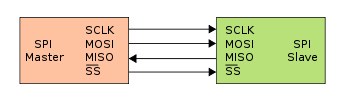
\includegraphics{Background/images/350px-SPI_single_slave.svg.png.png}
\caption{\citeauthor{FileSPIs48:online}, \citeyear{FileSPIs48:online}. \citetitle{FileSPIs48:online}}
\end{figure}
\vspace{1cm}
SPI has four main logic signals:
\begin{itemize}
\item SCLK: Serial clock, which accepts pulses obtained from the master
\item MOSI: Master Out Slave In, this is data transmitted from the master to slave
\item MISO: Master In Slave Out, this is data transmitted from the slave to master
\item CS/SS: Chip/Slave Select, an output from the master to notify data is being transmitted.
\end{itemize}
The RC522 module has 8 pins that interfaces with the Raspberry Pi;
\begin{itemize}
\item SDA: \gls{I2C}-bus serial data line input/output, it acts as a signal input when used for \gls{SPI} communication
\item SCK: \gls{SPI} serial clock input which has the same operation as SCLK
\item RST: an input for Reset and power-down of the module. It can turn off all the input pins and internal current sinks.
\item GND: for ground connection to the \gls{GPIO} pin of the master
\item IRQ: an interruption pin that could notify the master when an \gls{RFID} tag comes into the range of scan.
\item 3.3v/VCC: which powers the RC522 module
\item MOSI: has the same operation as MISO in \gls{SPI} communication. It receives data from master
\item MISO: has the same operation as MOSI in \gls{SPI} communication. It sends data to master(Raspberry Pi)
\end{itemize}
\subsubsection{Operations of \gls{RFID} module}
\gls{RFID} tags are classified by their frequencies, the four primary frequency ranges are:
\begin{itemize}
\item Low frequency (LF): they are frequencies from 30 to 300KHz
\item High frequency (HF): frequencies are from 3 to 30MHz, has a higher memory size and a longer range of transmission
\item Ultra high frequency (UHF): frequencies are from 300MHz to 3GHz
\item Microwave frequency (microwave): they function at 2.45GHz
\end{itemize}
\newacronym{PCD}{$PCD$}{Proximity coupling device}
\glsadd{PCD}
\newacronym{PICC}{$PICC$}{Proximity Integrated circuit card}
\glsadd{PICC}
The system consists of two main components, a transponder/tag and a transceiver/reader or a \gls{PCD} and a \gls{PICC} as defined in ISO 14443. The transceiver creates a 13.56MHz electromagnetic field that communicates with the tag.
This project uses a High Frequency passive card with Type A communication defined in ISO-14443, passive meaning, the tags only function when they acquire signals from a reader and relay an information-carrying signal back to the reader.
\subsection{Fingerprint - JM-101}
The JM-101 comes with a flash memory to store the fingerprints, it has a storage capacity of over 300 templates.
\subsubsection{Interfacing with Raspberry Pi}
The Fingerprint interfaces with the Raspberry Pi with \gls{UART} communication. \gls{UART} is a device that supports asynchronous serial communication, which is a form of serial communication that does not require a clock signal and is not constantly synchronized. Raspberry Pi supports asynchronous communication but with several fingerprints having distinct voltages. A USB to \gls{UART} Converter which supports both 3.3v and 5v was used although the JM-101 is compatible with a 3.3v pin. The TX pin goes to the RX pin and vice versa in the connection between the converter and fingerprint module. The USB to \gls{UART} Converter goes into the USB port of the Raspberry Pi while its pins are connected to the pins of the fingerprint module.
The pins used in interfacing with the \gls{UART} converter are:
\begin{itemize}
\item GND: ground connection
\item RXD: the receiver of data
\item TXD: transmits data
\item 3V3: powers the fingerprint module
\end{itemize}
\subsubsection{Operations of fingerprint module}
Fingerprint processing can either be for enrollment or matching. The user enters his finger two times when enrolling, the two templates are used to generate a template after processing their results.
A matching algorithm is used to compare fingerprint templates stored in the flash memory with the one read by the fingerprint module. There are two types of matching; 1:1 and 1:N. In 1:1 the module compares the read fingerprint with a pre-existing template that is specified in the code while \label{fingerprint 1:N}1:N checks the read fingerprint with all templates previously stored in the flash memory.
\subsection{Flask}
This creates a local web server written in python. It has a feature that binds a python function to a \gls{URL} endpoint. Another feature of flask is its ability to handle multiple requests with one function. It is in the form of a switch or if-else condition: if it is a POST it executes a codeblock but if it is a GET it executes another codeblock.
\subsection{Virtual tunnel}
Pitunnel is used to connect the Flask server with the NodeJS server that is used for development purposes. The Flask server alone runs locally and has no access to the Internet. Pitunnel is a service that allows access to any network service on the Raspberry Pi from anywhere in the world. In this project the service used is \gls{HTTP}. All that is required is to configure pitunnel to track the localhost server running and you one use the pitunnel endpoint to receive data on the Raspberry Pi. Pitunnel does this by mirroring the flask server: the root directory of the flask server becomes the root directory of the Pitunnel same as other endpoints when calling an endpoint of the flask server.
\section{Cloud - Azure}
Cloud computing has to do with the provision of computing system resources like data storage, servers, software over the internet\cite{Cloudcom53:online}. The benefits of these include reliability: the cloud provider is in charge of handling data and handles data back-up by mirroring these data at different locations, Scalability: the ability for you to "scale up" when there is an increase in demand for computing power. Scalability ensures the appropriate amount of resources for a task is provided. 
There are different types of clouds and they have unique functions;
\begin{itemize}
\item Public cloud: Public clouds  are delivered over the internet by third-party providers like Microsoft Azure, Amazon Web Services etc.
\item Private cloud: Private cloud resources are solely designed for a single organisation. These resources can be handled by a third-party or hosted by that organisation and located on their own personalised data centre.
\item Hybrid cloud: a combination of a private and public cloud and aims to give the user more flexibility. An organisation could host a private cloud with sensitive data and connect with a public cloud to host its application
\end{itemize}
\newacronym{IaaS}{$IaaS$}{Infrastructure as a service}
\glsadd{IaaS}
\newacronym{PaaS}{$PaaS$}{Platform as a service}
\glsadd{PaaS}
\newacronym{SaaS}{$SaaS$}{Software as a service}
\glsadd{SaaS}
These clouds provide their services according to models, there are mainly three according to \cite{National47:online};
\begin{figure}[h]
\centering
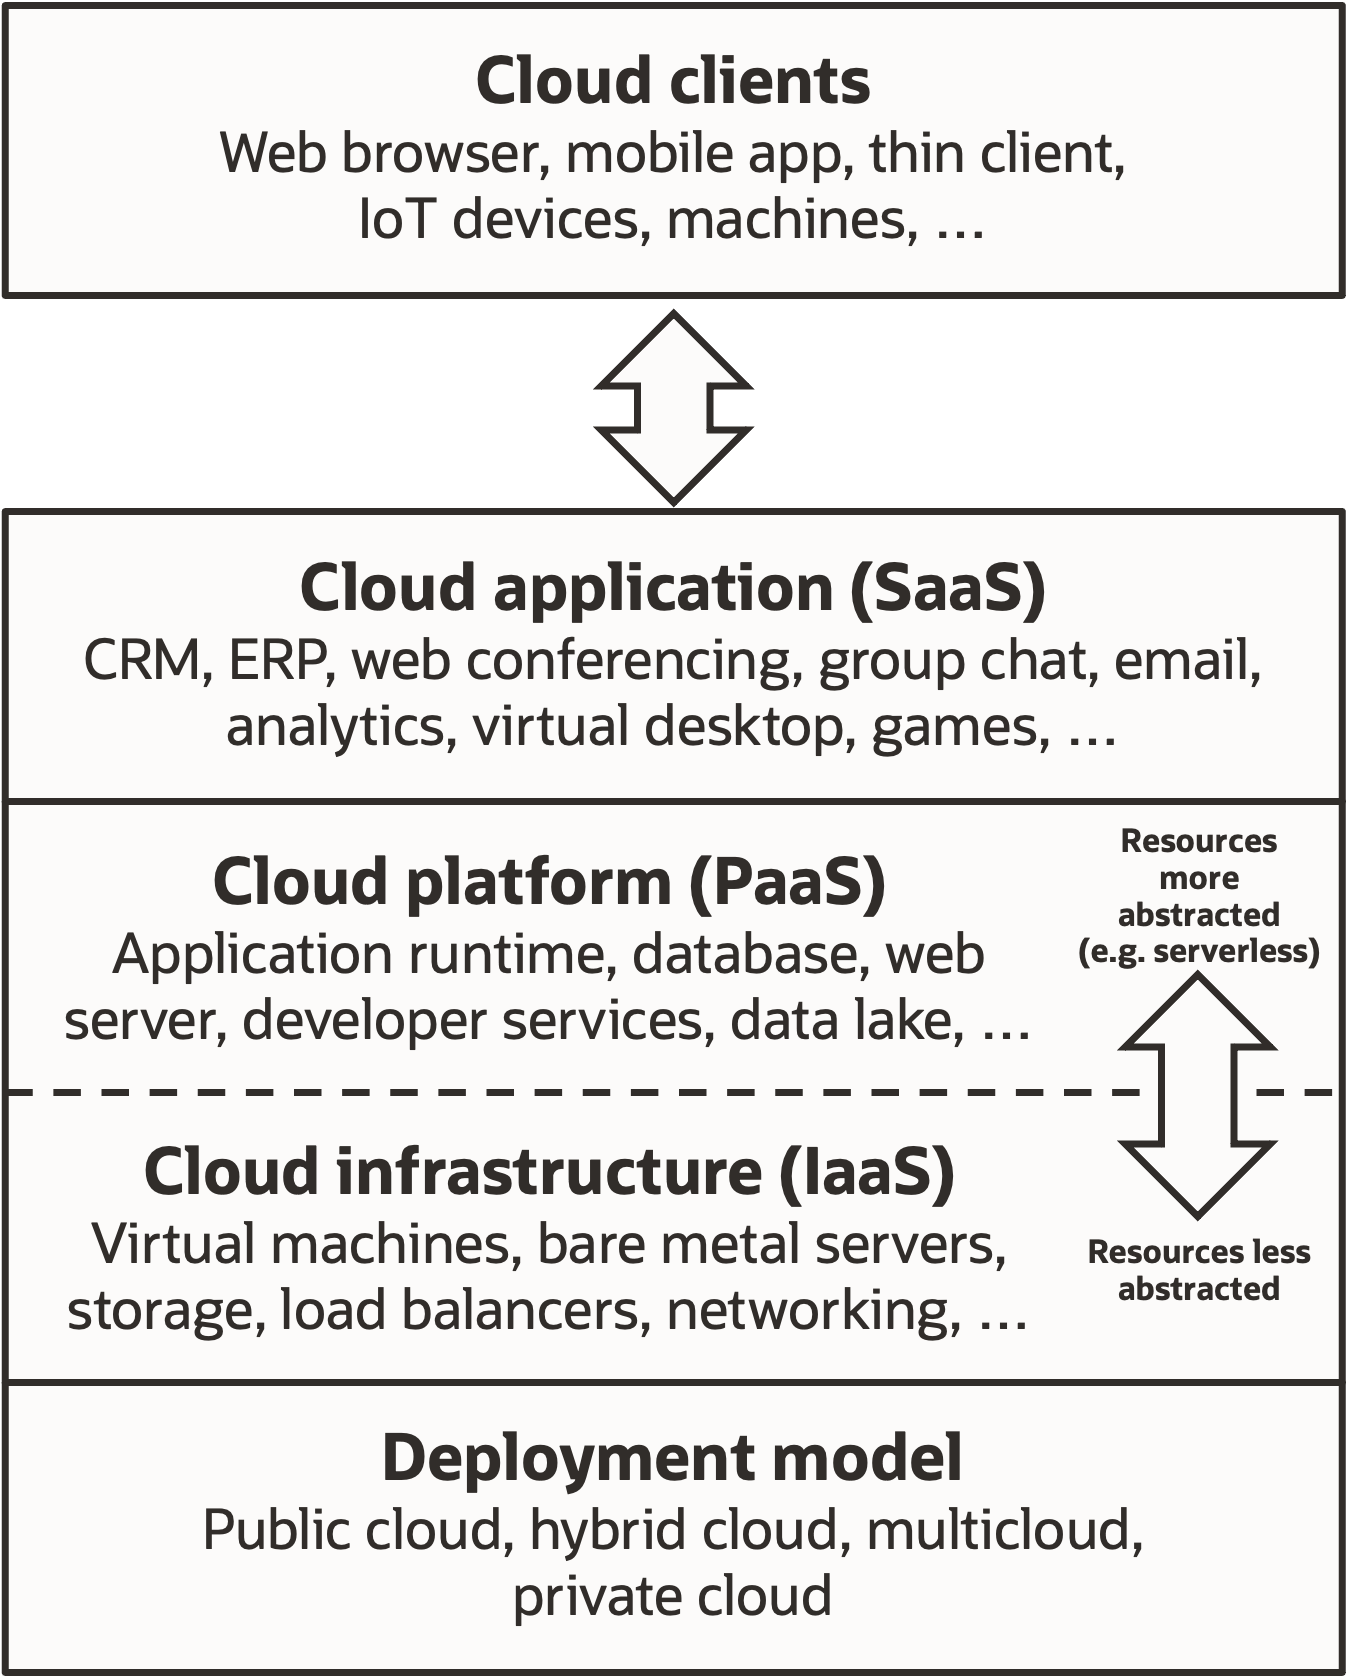
\includegraphics[scale=0.8]{Background/images/Cloud_computing_service_models_(1).png}
\caption{\citeauthor{FileClou30:online}, \citeyear{FileClou30:online}. \citetitle{FileClou30:online}}
\end{figure}
\begin{itemize}
  \item \gls{IaaS}: this provides the user with resources like virtual machines, storage, operating systems
  \item \gls{PaaS}: provides the user with an environment to develop software without management of the underlying resources required like servers, operating systems
  \item \gls{SaaS}: the cloud provider supply users with software over the Internet, this is mostly done by connection to a web browser, here the consumer does not management the underlying resources
\end{itemize}
This project uses a public cloud type provided by Microsoft Azure and \gls{IaaS} for the storage and \gls{PaaS} for the server. AzureSQL server hosts the SQL database and handles connection to other devices, programs or services.
My options were NoSQL("Not Only SQL") or SQL also known as Sequel.
SQL is a programming language used to manage data in a relational database. T-SQL was specifically used for querying data in Microsoft SQL Server.




\subsection{Terms Used}[h]
A lot of these terms will be used to talk about managing the database;
\begin{itemize}
\item Table: Tables contain all data in database, they do this in the form of a row and column format, where each row is a unique record and each column a unique attribute
\item Rows: represents a collection of attributes that make up a data record
\item Columns: Columns represent different attributes of a table. They can also be called fields or attributes. a single column has a similar data type for all rows.
\item Primary key: A primary key is a column or a group of columns that acts as an identifier of each row of a table.
\item Foreign key: A foreign key can be a column or a group of columns that allows a link between two related tables by referring to the Primary Key of another table
\item Database relationships: database tables sometimes share certain relationships with each other. This relationship can be represented in mainly three ways;
 \begin{itemize}
   \item one-to-one relationship: a one-to-one is when both tables have only online record stored on each side. One record in a table relates to one and only one record in the other table and vice versa.
   \item one-to-many relationship: When the primary-key table can relate to zero to many records in another table.
   \item many-to-many relationship: each records in both tables can relate to none and above in the other table.\label{manytomany} Most relational database systems do not support this relationship and a third table is used to link the both tables to each other.
\end{itemize}
\end{itemize}
 
 
 
\subsection{Communication between the Database and other devices}
The azure web portal provides a list of connection strings to interact with the sql database. For this project ODBC driver was used with SQL authentication connection string:
\begin{verbatim}
Driver={ODBC Driver 13 for SQL Server};
Server=tcp:csproj.database.windows.net,1433;
Database=vantracker;
Uid=g3ar;
Pwd={your_password_here};
Encrypt=yes;
TrustServerCertificate=no;
Connection Timeout=30;
\end{verbatim}
 
 The Design \& Implementation explain the choices taken for each part of the system and why they were chosen.
 
 

